\chapter{Hardware Implementation}\label{quantization}
In this chapter, the hardware-aware optimizations used in the FPGA implementations are first presented and then their application in the proposed architectures is explained. Other elements of the hardware design and configuration process are then described which results in a comprehensive picture of the FPGA-mapped architectures. Afterwards, two analytical models are considered - one for the latency and the other for the resource utilization. The custom post-training quantization tool is discussed along with its suitability for this project. Then, existing infrastructure that ties together higher and lower-level code representation is introduced along with its synergy with a High-Level Synthesis optimization tool chain. Lastly, the technical contributions to \hlsml library are listed and explained.

\section{Hardware-Aware Optimizations}

\subsection{Tensor Multiplication and Scaling}
Each self-attention head performs two tensor multiplications (referred to as \textit{matmul} blocks in figure \ref{fig:self-attention-multi-head}), which are normally expressed using Einstein Summation notation \cite{59-barr1991einstein}, which is supported by mathematical and machine learning libraries like \texttt{NumPy} or \texttt{PyTorch}. However, not present by default in HLS, it requires careful design of the calculation loops in order to not cripple the performance by unnecessary computations and pseudo-random data accesses. As part of this research, an efficient and fully-customizable HLS block has been designed, that uses a very similar interface to the Python equivalent.

\begin{figure}[hpt!]
  \centering
  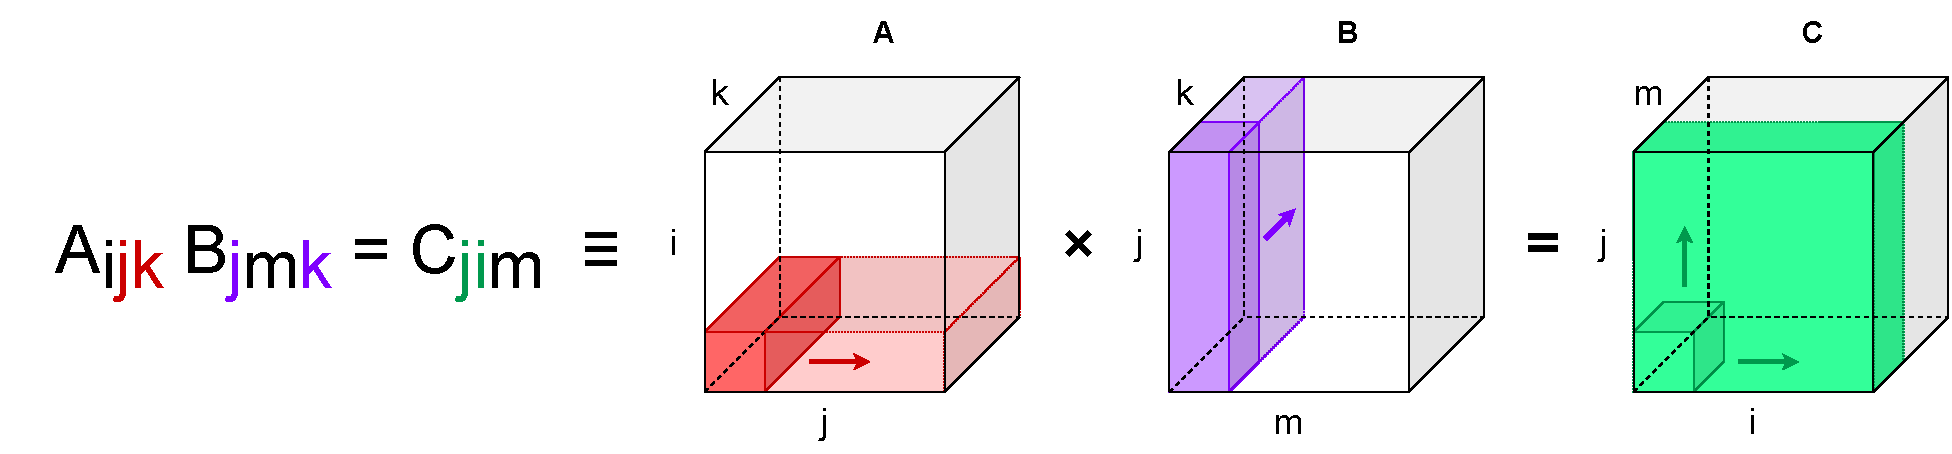
\includegraphics[trim={0cm 0cm 0cm 0cm}, width=0.75\textwidth, center]{models/einsum.pdf}
  \caption{Visualization of a tensor operation expressed in Einstein Summation notation.}
  \label{fig:einsum}
\end{figure}

Figure \ref{fig:einsum} shows a visualization for an example notation to give a better understanding of the necessary flexibility of a formula. The translation between notations using the custom tool is showcased in listing \ref{list:einsum}. While the \texttt{PyTorch} implementation can often use 4-dimensional tensors, the first dimension refers to the batch, which is not present in the hardware implementation that processes input samples one-by-one, hence both the figure and code listing show 3-dimensional cases. It is also worth pointing out, that tensor multiplication is an inherently computationally expensive operation due to the quadruple-nested loop structure. For this reason, the proposed design leaves the configuration of pipelining as a parameter that offers a trade-off between time and design complexity. The \textit{design} complexity refers to the difficulty involved in HLS synthesis as well as hardware resource utilization. In other words, the hardware block can be instantiated to run serially, where little resources are needed as they get re-used, or alternatively, in parallel, where significantly more components are used to decrease latency, and in case the design is also pipelined, to also increase throughput.

% \clearpage
\lstinputlisting[language={[GNU]C++}, caption={From PyTorch \texttt{out = torch.einsum("qhc,khc->hqk", [A, B])} to HLS C++ code.}, captionpos=b, label={list:einsum}]{quantization/einsum_example.cpp}

\begin{equation}\label{eq:einsum-no-unrolling}
  \text{Design}: \mathcal{O}(n) \quad \text{Time}: \mathcal{O}(HKQC \cdot n)
\end{equation}

Let's consider the two extreme cases for the design - no loop unrolling and complete unrolling, where the latter is required for the block to be fully pipelined, and assume that multiply-accumulate and addition both have \(n\) time and space complexity. In the first case, a single multiply-accumulate operation happens at once, hence a final result is only available after all the loops have been fully iterated, with complexities shown in \ref{eq:einsum-no-unrolling}.

\begin{equation}\label{eq:einsum-full-unrolling}
  \text{Design}: \mathcal{O}(HKQC \cdot n) \quad \text{Time}: \mathcal{O}(n \cdot \log (HKQC))
\end{equation}

In the second one, all loop operations can execute at the same time, although the intermediate results need to be summed accordingly using an adder tree (seen in figure \ref{fig:adder-tree}) which has a logarithmic time and linear space complexity, before saving the output tensor, which leads to complexities seen in \ref{eq:einsum-full-unrolling}. The time complexity may appear high, but it has to be remembered that unrolling allows for the pipelining of this design, which cannot decrease latency, but can vastly increase throughput, as each addition can happen in a single cycle.

\begin{figure}[hpt!]
  \centering
  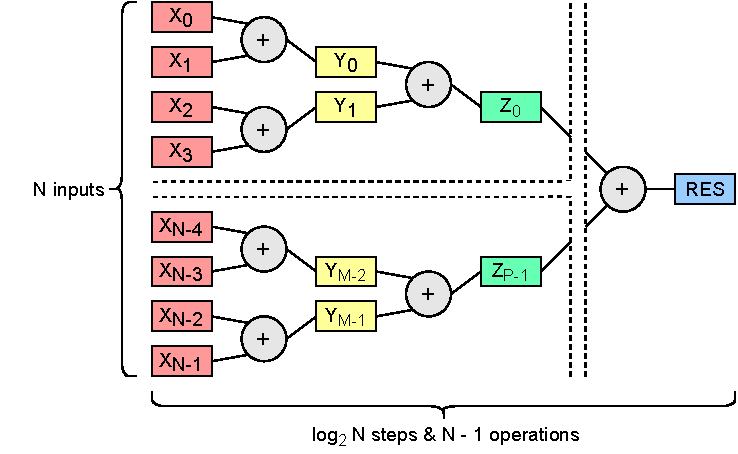
\includegraphics[trim={0cm 0cm 0cm 0cm}, width=0.51\textwidth, center]{quantization/adder_tree.pdf}
  \caption{Illustration of an adder tree with \(N\) inputs.}
  \label{fig:adder-tree}
\end{figure}

Another simple optimization used alongside the tensor multiplication blocks was the change in size scaling from using division to performing an arithmetic right shift (ASR), which requires precomputing the logarithm of the size, seen in equation \ref{eq:log-div}, vastly simplifying the otherwise computationally expensive hardware required at run-time.

\begin{equation}\label{eq:log-div}
  \frac{x}{\sqrt{\text{size}}} \equiv \text{ASR}(x,\; \log_2 \sqrt{\text{size}}) \equiv \text{ASR}(x,\; \frac{1}{2}\log_2 \text{size})
\end{equation}


\subsection{Softmax and Log Softmax Activations}
Despite an already existing \hlsml implementation of the softmax activation function, computing the logarithm of its result is not as simple as it may seem. This is because the numerical stability and computational efficiency of this operation is often explored in-depth \cite{60-blanchard2019accurate} and varies depending on the programming language and target platform.

\begin{figure}[hpt!]
  \centering
  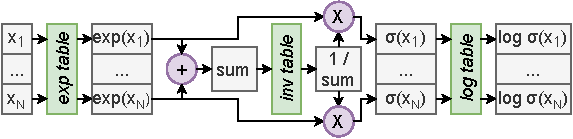
\includegraphics[trim={0cm 0cm 0cm 0cm}, width=0.55\textwidth, center]{quantization/log_softmax_naive_h.pdf}
  \caption{Direct hardware implementations of log softmax.}
  \label{fig:log-softmax-naive}
\end{figure}

The naive implementation comes straight from the definition of taking a logarithm of softmax, seen in equation \ref{eq:softmax}, and the required hardware operations are shown in figure \ref{fig:log-softmax-naive}.

\begin{equation} \label{eq:softmax}
    \sigma (x_i) = e^{x_i} / \sum_{j=1}^{N} e^{x_j}
\end{equation}

This report proposes a different way of mapping this operation to hardware to improve stability while shortening the critical path and using less resources. It is based on the derivation shown in equation \ref{eq:log-softmax}.

\begin{equation} \label{eq:log-softmax}
    \log (\sigma (x_i)) = log(e^{x_i} / \sum_{j=1}^{N} e^{x_j}) = \log(e^{x_i}) - \log(\sum_{j=1}^{N} e^{x_j}) = e^{x_i} - \log(\sum_{j=1}^{N} e^{x_j})
\end{equation}

The resulting hardware operations are depicted in figure \ref{fig:log-softmax-opt}. It is important to note, that operations like exponentiation, division or taking a logarithm usually rely on precomputing a wide range of values and mapping them in BRAMs or LUTs to allow for lookup on run-time. Hence, the optimized design requires one less of such lookups while also replacing multiplication by a subtraction, which can be simpler to express in hardware.

\begin{figure}[hpt!]
  \centering
  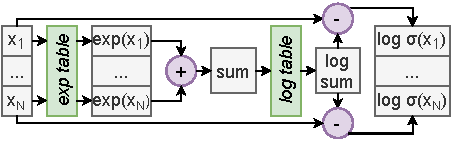
\includegraphics[trim={0cm 0cm 0cm 0cm}, width=0.5\textwidth, center]{quantization/log_softmax_opt_h.pdf}
  \caption{Optimized hardware implementations of log softmax.}
  \label{fig:log-softmax-opt}
\end{figure}

\clearpage
Although further simplifications, including approximating the summation by finding the maximum (see equation \ref{eq:log-softmax-max}) or simply omitting the logarithm portion of the expression, were also explored, they noticeably lowered the final accuracy and were thus abandoned. \todo{Confirm if page breaks correctly.}

\begin{equation} \label{eq:log-softmax-max}
    \log (\sigma (x_i)) = e^{x_i} - \log(\sum_{j=1}^{N} e^{x_j}) = e^{x_i} - \sum_{j=1}^{N} \log(e^{x_j}) = e^{x_i} - \sum_{j=1}^{N} x_j \approx e^{x_i} - \max(x)
\end{equation}


\section{Neural Network Architectures Design}
\indo{|}
\indo{|}
\indo{|}

\subsection{Ultra-Low Latency Architecture}
\indo{|}
\indo{|}
\indo{|}
\indo{|}
\indo{|}
\indo{|}

\subsection{Accuracy-Focused Architecture}
\indo{|}
\indo{|}
\indo{|}
\indo{|}
\indo{|}
\indo{|}


\section{Analytical Latency and Resource Models}
\indo{Reason about computational complexity, include a diagram of self-attention tensor multiplications based on contents of Deep Learning lectures}
\indo{|}
\indo{|}
\indo{|}
\indo{|}
\indo{|}
\indo{|}
\indo{Derive simple latency and resource (likely only DSP as others are too difficult) model, that will be verified in evaluation chapter}
\indo{|}
\indo{|}
\indo{|}
\indo{|}


\section{Post-training Quantization}\label{post-training-quantization}
This section returns to the topic of quantization, but as opposed to \cref{pre-training-quantization}, it explores the quantization of already trained models. This is domain is not researched as much as quantization-aware training due to the lack of ability for a model to \textit{compensate} for the quantization noise during training, hence leading to potentially inferior results. However, recent advancements in this field \cite{80-wang2019haq:} leverage the synergy between post-training quantization and the target hardware platform to produce results with improved latency or energy consumption. The inherent noise issues are offset by a careful per-variable bit-width analysis, driven by a reinforcement learning algorithm. The choice of the algorithm has a deep-rooted issue for more computationally demanding models that also require a search in a wider range of bit-widths\footnote{The mentioned method only explores convolutional neural networks in \([1, 8]\) bit-width range.}.

\subsection{Motivation}
This report proposes a novel post-training quantization algorithm that can be applied to state-of-the-art transformer neural networks over a wide precision range. Early tests in the HLS environment revealed that a single C simulation for an input with only 100 samples can take around 10 minutes, which dictates a need for a significantly simpler, hence faster, algorithm than Bayesian optimization or reinforcement learning to allow for an exploration that runs in a reasonable amount of time.

The motivation of the algorithm comes from a hypothesis which states that the neighboring layers in a neural network have a relatively high correlation in their optimal bit-widths. Under this assumption, each layer's input, output, weight, bias and accumulator can be safely explored one-by-one, in the order of appearance in the model. \textit{Safely} refers here to a low likelihood of arriving at a local accuracy extremum that is substantially worse than the global one, that could only theoretically be found using a more sophisticated approach. During this \textit{walk} through the design space, several non-trivial constraints about the widths have to be ensured, which are the topic of the next subsection.

\subsection{Constraints}
The constraints of a network variable could theoretically be set arbitrarily to convey a high-level requirement of an experienced designer with a knowledge about typical widths used for a component in a given network type. However, the proposed method automates this process by extracting the underlying lookup table characteristics to accommodate users without domain-specific expertise. These characteristics are part of the network configuration that ensures that any precomputed (for increased latency) function is stored with adequate precision that avoids introducing unnecessary errors. To give a more concrete example to this abstract definition, one can consider the range of values yielded from the exponential function. Not only is there a set width for the results, but even relatively small values map to numbers that require several bits of integer precision, so careless reduction to either of the width parts can quickly degrade any learning capacity of the model.

\begin{figure}[hpt!]
  \centering
  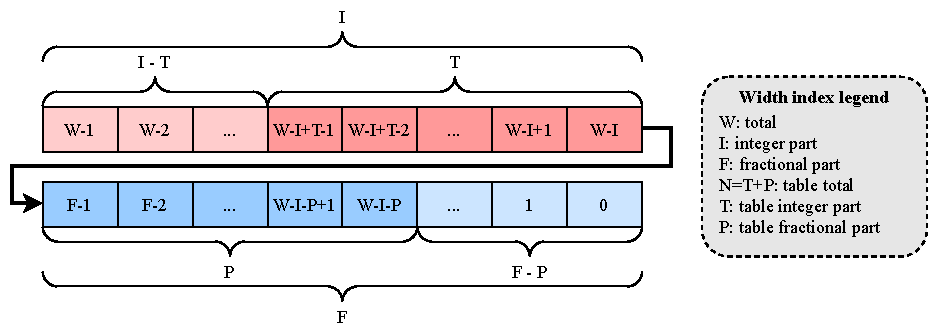
\includegraphics[trim={0cm 0cm 0cm 0cm}, width=1.0\textwidth, center]{quantization/width_constraints.pdf}
  \caption{Visualization of a fixed-point number with its bit-widths as well as constraints imposed by a lookup table. For convenience, red and blue distinguish integer and fractional parts, while the darker hue shows the table-related parts.}
  \label{fig:width-constraints}
\end{figure}

Figure \ref{fig:width-constraints} visualizes a fixed-point number with a detailed analysis of its structure in terms of lookup table constraints. At first, it could be assumed that the imposed widths should simply be adopted by the variables used by the corresponding table values. However, it is possible for such variables to also have connections to other paths in a network, which can require more precision than the table, hence justifying the existence of the constraints ranges presented in equations \ref{eq:width-constraint-1}, \ref{eq:width-constraint-2}, and \ref{eq:width-constraint-3}, with the notation coming from the corresponding figure.

\begin{equation} \label{eq:width-constraint-1}
  W \geqslant N > T \geqslant 1
\end{equation}
\begin{equation} \label{eq:width-constraint-2}
  W \geqslant I \geqslant T \geqslant 1
\end{equation}
\begin{equation} \label{eq:width-constraint-3}
  W \geqslant F \geqslant P \geqslant 1
\end{equation}

\subsection{Steps}



It is important to point out that the aforementioned PyTorch Eager Mode and FX Graph Mode quantization schemes offer post-training quantization, but there are unsuitable for this work due to their lack of flexibility and support for the essential neural network layers.

\indo{Walk through the steps and explain the parameters, pointing to provided algorithm}
\indo{Talk about correlation of neighboring bit widths and how this is exploited (i.e. by resuming with previous width + the whole idea is based on that instead of a full gradient descent style search)}

\begin{algorithm}
  \caption{Algorithm for performing post-training quantization search}\label{alg:post-training-quant}
  \begin{algorithmic}
  \Function{PostTrainingQuantization}{neg\_accuracy\_tolerance, pos\_accuracy\_tolerance}

  \State $previous\_width \gets null$
  \State $max\_decrement \gets neg\_accuracy\_tolerance \cdot 2$ \Comment{Maximum decrement per parameter}
  \State $optimal\_accuracy \gets$ find\_accuracy()
  \State $params \gets$ scan\_file($defines\_file$) \Comment{FIFO with scanned parameter objects}

  \While{$params$ not empty}
    \State $current \gets params$.pop()

    \If{$previous\_width$ exists} \Comment{Try using width from previous parameter}
      \State $original\_width \gets params.width$
      \State update($params$, $previous\_width$)
      \If{find\_accuracy() $< optimal\_accuracy - max\_decrement$}
        \State update($params$, $original\_width$)
      \Else
        \State $optimal\_accuracy \gets$ find\_accuracy()
      \EndIf
    \EndIf

    \For{$part$ in $\{int, frac\}$}

      \State $try\_increase \gets True$
      \State $pos\_improvement\_found \gets False$
      \While{$try\_increase$} \Comment{Increment to check for high accuracy gain}
        \State $param$.increment($part$)
        \If{find\_accuracy() $ > optimal\_accuracy + pos\_accuracy\_tolerance$}
          \State $optimal\_accuracy \gets$ find\_accuracy()
          \State $pos\_improvement\_found \gets True$
        \Else
          \State $try\_increase \gets False$
          \State $param$.decrement($part$)
        \EndIf
      \EndWhile

      \If{not $pos\_improvement\_found$} \Comment{Decrement if no good increment}
        \State $try\_decrease \gets True$
        \State $acc\_before\_decrease \gets optimal\_accuracy$
        \While{$try\_increase$}
          \State $param$.decrement($part$)
          \If{$acc\_before\_decrease -$ find\_accuracy()$ > max\_decrement$}
            \State $try\_decrease \gets False$
            \State $param$.increment($part$)
          \ElsIf{find\_accuracy() $ > optimal\_accuracy - neg\_accuracy\_tolerance$}
            \State $optimal\_accuracy \gets$ find\_accuracy()
          \Else
            \State $try\_decrease \gets False$
            \State $param$.increment($part$)
        \EndIf
        \EndWhile
      \EndIf
    \EndFor
  \EndWhile
  \State \textbf{return} $params$
  \EndFunction
  \end{algorithmic}
\end{algorithm}


\section{High-Level-Synthesis Optimization}
\indo{Introduce MLIR and the overall flow of how PyTorch models are mapped, include nice diagrams}
\indo{|}
\indo{|}
\indo{|}
\indo{|}
\indo{|}
\indo{Talk about how ScaleHLS extends MLIR to HLS, again diagrams}
\indo{|}
\indo{|}
\indo{|}
\indo{|}
\indo{|}
\indo{Talk about potential integration/relation between hls4ml (Python -> HLS) and ScaleHLS (PyTorch/HLS -> Optimized HLS) }
\indo{|}
\indo{|}


\section{\hlsml Contributions}
In this section, the technical contributions to the \hlsml library are descriptively presented, highlighting the areas that this work expands upon. Developed components are shown in figure \ref{fig:hls4ml-contributions}, along with a number of existing components that were expanded upon or are used to draw comparison with. Each group is discussed in the following subsections.

\begin{figure}[hpt!]
  \centering
  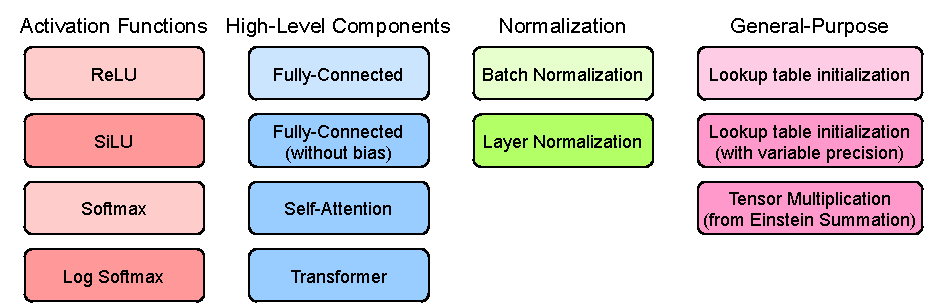
\includegraphics[trim={0cm 0cm 0cm 0cm}, clip, width=0.7\textwidth, center]{evaluation/hls4ml_blocks.pdf}
  \caption{Overview of the created implementations (dark-colored) and some existing components with similar functionality (light-colored).}
  \label{fig:hls4ml-contributions}
\end{figure}


\subsection{Activation Functions}
\indo{Mention SiLU which was experimented with}
\indo{Mention Log Softmax that implements the architecture from previous chapter}
\indo{|}
\indo{|}

\subsection{High-Level Components}
\indo{Briefly mention FC without bias as an optimization that saves initializing accumulators with bias values}
\indo{Talk in details about the C++ HLS challenges and achievements of self-attention and transformer}
\indo{|}
\indo{|}
\indo{|}
\indo{|}


\subsection{Normalization Layers}
\indo{Discuss how layer norm and batch norm actually differ}
\indo{|}
\indo{|}


\subsection{General-Purpose Blocks}
\indo{Explain the mechanism of function look up table initialization and how it was automatic}
\indo{|}
\indo{Show when automatic precision/range fails and how the new block addresses that by exposing int bit width as a parameter}
\indo{|}
\indo{|}
\indo{|}
\indo{Mention tensor einsum and the pragmas it uses}
\indo{|}

